\section{Environnement Linux Embarqué}
\subsection{Objectifs}
\noindent
Ce travail pratique vise les objectifs suivants:
\begin{enumerate}
	\item Mise en œuvre d'un système embarqué sous Linux
	\item Mise en oeuve de l'environnement de développement de systèmes embarqués sous Linux
	\item Debugging d'applications sous Linux embarqué
	\item Mise en production d'un système embarqué sous Linux
\end{enumerate}
\subsection{Informations pratiques}
Nous avons choisi l'option de travailler directement avec la machine virtuelle fournie.
\subsection{Gravure de la carte SD}
Avant de pouvoir graver la carte, il faut trouver le nom du périphérique auquel elle est attachée. Il peut être obtenu avec la commande suivante:
\begin{lstlisting}
$ mount
...
/dev/sd2 on /media/lmi/usrfs type ext4 (rw,nosuid,nodev,uhelper=udisks2)
/dev/sd1 on /media/lmi/5a13f590-5792-413e-ba62-403debdf56a5 type ext4 (rw,nosuid,nodev,uhelper=udisks2)
...
\end{lstlisting}
La commande va lister tous les périphériques connectés, dans notre cas, la carte SD se nomme lmi et est liée à /dev/sdb2 et /dev/sdb1.\\
Un script a ensuite été écrit, regroupant les différentes commandes à exécuter pour la gravure de la carte.\\\\
\textbf{Emplacement du script : } \textit{/EnvLinuxEmbarque/flasheMMC.sh}\\\\
Le plus simple est de placer le script directement dans le workspace CSEL. Il s'exécute à l'aide de la commande suivante:
\begin{lstlisting}
./flasheMMc.sh
\end{lstlisting}
Il va aller détacher les volumes attachés à la carte SD, créer la table de partition et graver les différents firmwares et images.\\
\\
Une fois la carte gravée et insérée dans la cible, le ventilateur se met à tourner si tout s’est bien passé. Si rien ne se passe, il faut également contrôler que le switch de l’Odroid est dans la position pour booter sur la carte SD.
\subsection{Mise en place de l'infrastructure}
La cible ODROID-XU3 doit avoir l’adresse IP 192.168.0.11 et la machine hôte l’IP 192.168.0.4.
\subsubsection{Configuration de la machine virtuelle}
Pour associer la carte réseau de l’ordinateur à la machine virtuelle, il faut suivre les étapes ci-dessous :
\begin{enumerate}
	\item Éteindre la vm, aller dans\textit{ edit->Virtual Network Editor…->change settings}
	\item Dans la fenêtre des réseaux, changer la configuration en bridged to : Il faut choisir la carte réseau de l'ordinateur. Ici, Contrôleur PCIe (propre à l’ordinateur).
\end{enumerate}
\begin{figure}[H]
	\begin{center}
		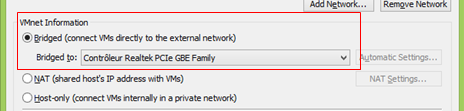
\includegraphics[width=14cm]{img/vmConfig1.png}
		\caption{Configuration de la carte réseau}
		\label{evLinuxConfig1}
	\end{center}
\end{figure}
Puis dans les settings de la VM, il faut aller changer le réseau pour utiliser celui que l’on vient de configurer.
\begin{figure}[H]
	\begin{center}
		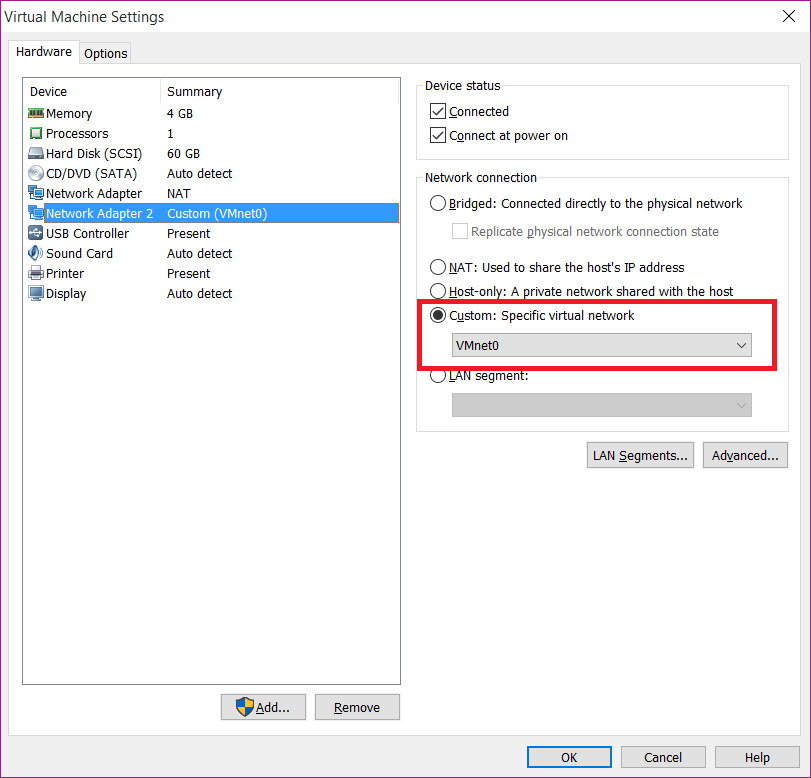
\includegraphics[width=14cm]{img/vmConfig2.png}
		\caption{Association de la carte réseau à la machine virtuelle}
		\label{evLinuxConfig2}
	\end{center}
\end{figure}
La dernière étape est d’activer le réseau dans la machine virtuelle (icône réseau -> enabling networking).
\begin{figure}[H]
	\begin{center}
		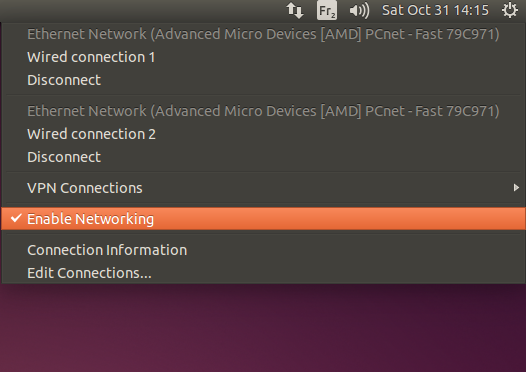
\includegraphics[width=14cm]{img/vmConfig3.png}
		\caption{Activation du réseau}
		\label{evLinuxConfig3}
	\end{center}
\end{figure}

\subsubsection{Accès ssh sans mot de passe}
Il faut aller modifier le fichier \textit{/etc/ssh/sshd\_config} sur la cible pour autoriser l’accès sans mot de passe.\\ Pour accéder au fichier, il faut entrer sur la cible par la connexion série :
\begin{lstlisting}
$ sudo minicom

Welcome to minicom 2.7

OPTIONS: I18n 
Compiled on Jan  1 2014, 17:13:22.
Port /dev/ttyUSB0, 13:10:43

Press CTRL-A Z for help on special keys


Welcome to Hardkernel ODROID_XU3 board
odroidxu3 login: root
# 

\end{lstlisting}
On peut ensuite rechercher le fichier et l’éditer avec vi ou vim pour changer l'attribut suivant à "yes": "PermitEmptyPassword yes". Il faut ensuite redémarrer la cible :
\begin{lstlisting}
# reboot
\end{lstlisting}
Normalement, on devrait avoir accès à la cible en ssh en entrant la commande suivante dans la machine hôte :
\begin{lstlisting}
lmi@csel1:~$ ssh root@192.168.0.11
# 
\end{lstlisting}
Pour valider la connexion Ethernet/IP, on peut également arrêter la cible dans son U-boot en tapant la touche "carriage return" et faire un ping de la machine hôte:
\begin{lstlisting}
lmi@csel1:~$ sudo minicom
...
# reboot
...                                                      
Press 'Enter' or 'Space' to stop autoboot:  0       
                            
ODROIDXU3> usb start                                                          
(Re)start USB...                                                                
...    

ODROIDXU3> ping 192.168.0.4                                                     
Waiting for Ethernet connection... done.                                        
Using sms0 device                                                               
host 192.168.0.4 is alive

ODROIDXU3> run nfsboot
\end{lstlisting}
Si la machine hôte répond au ping, tout a bien été configuré. La dernière commande "run nfsboot" permet de démarrer la cible en mode développement.

\subsubsection{Création de l'espace de travail}
Le but est de partager le répertoire de projet de la machine hôte avec la cible. Pour cela, il faut accéder à la cible via le port série ou par ssh et taper les commandes indiquées dans la donnée. Celles ci-dessous montrent comment attacher automatiquement l'espace de travail.
\begin{lstlisting}
# mkdir /usr/workspace
# vi /etc/fstab
	# /etc/fstab: static file system information.
	#
	# <file system> <mount pt>     <type>   <options>         <dump> <pass>
	/dev/root       /              ext2     rw,noauto         0      1
	proc            /proc          proc     defaults          0      0
	devpts          /dev/pts       devpts   defaults,gid=5,mode=620   0      0
	tmpfs           /dev/shm       tmpfs    mode=0777         0      0
	tmpfs           /tmp           tmpfs    mode=1777         0      0
	sysfs           /sys           sysfs    defaults          0      0
	192.168.0.4:/home/lmi/workspace /usr/workspace  nfs     hard,intr,nolock
# mount -a
# reboot
\end{lstlisting}
Pour contrôler que le répertoire est bien partagé avec la cible, on peut y entrer la commande mount et normalement on voit le répertoire partagé. Il sera maintenant attaché automatiquement à chaque démarrage de la cible en mode de développement.
\begin{lstlisting}
# mount
...
192.168.0.4:/home/lmi/workspace on /usr/workspace type nfs (rw,relatime,vers=3,rsize=131072,wsize=131072,namlen=255,hard,nolock,proto=tcp,timeo=600,retrans=2,sec=sys,mountaddr=192.168.0.4,mountvers=3,mountproto=tcp,local_lock=all,addr=192.168.0.4)
\end{lstlisting}
\subsection{Debugging de l'application}
Cette section présente les différentes étapes à réaliser pour configurer l'environnement Eclipse pour qu’il utilise une connexion ssh entre l’hôte et la cible et pouvoir debugger à distance une application.
Pour cela, il faut commencer par charger un projet dans Eclipse :
\begin{enumerate}
	\item File -> Import… (si le projet existe déjà)
	\item C/C++ ->Existing Code as Makefile Project (configure pour utiliser le Makefile du projet et non celui généré par Eclipse)
\end{enumerate}
Une fois le projet importé dans l’espace de travail, il faut configurer le debugger:
\begin{figure}[H]
	\begin{center}
		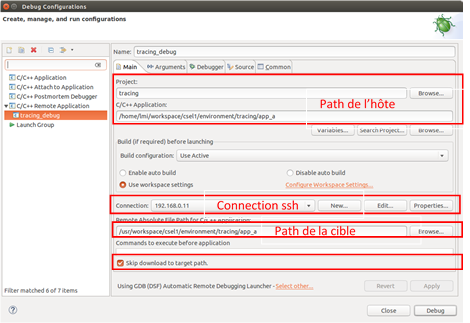
\includegraphics[width=16cm]{img/eclipseConfig1.png}
		\caption{Configuration du debugger}
		\label{eclipseConfig1}
	\end{center}
\end{figure}
Pour pouvoir entrer le path de la cible, il faut impérativement que la connexion ssh soit configurée comme ci-dessous :
\begin{figure}[H]
	\begin{center}
		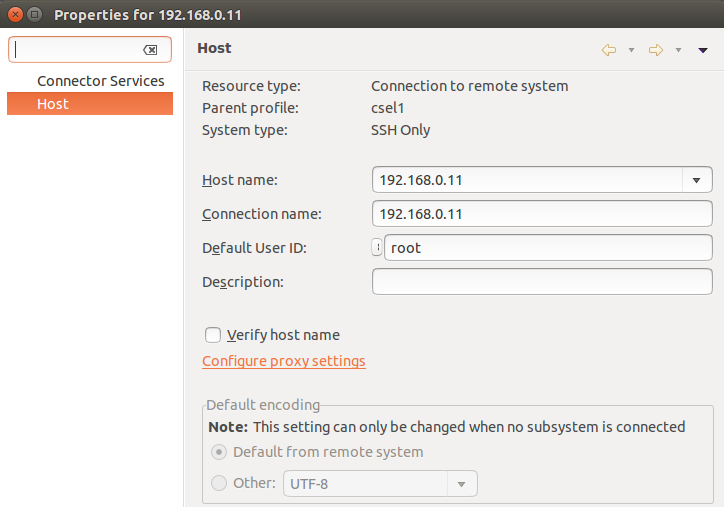
\includegraphics[width=15cm]{img/eclipseConfig2.png}
		\caption{Configuration de l'accès ssh}
		\label{eclipseConfig2}
	\end{center}
\end{figure}
Il faut encore aller configurer le debugger gdb :
\begin{figure}[H]
	\begin{center}
		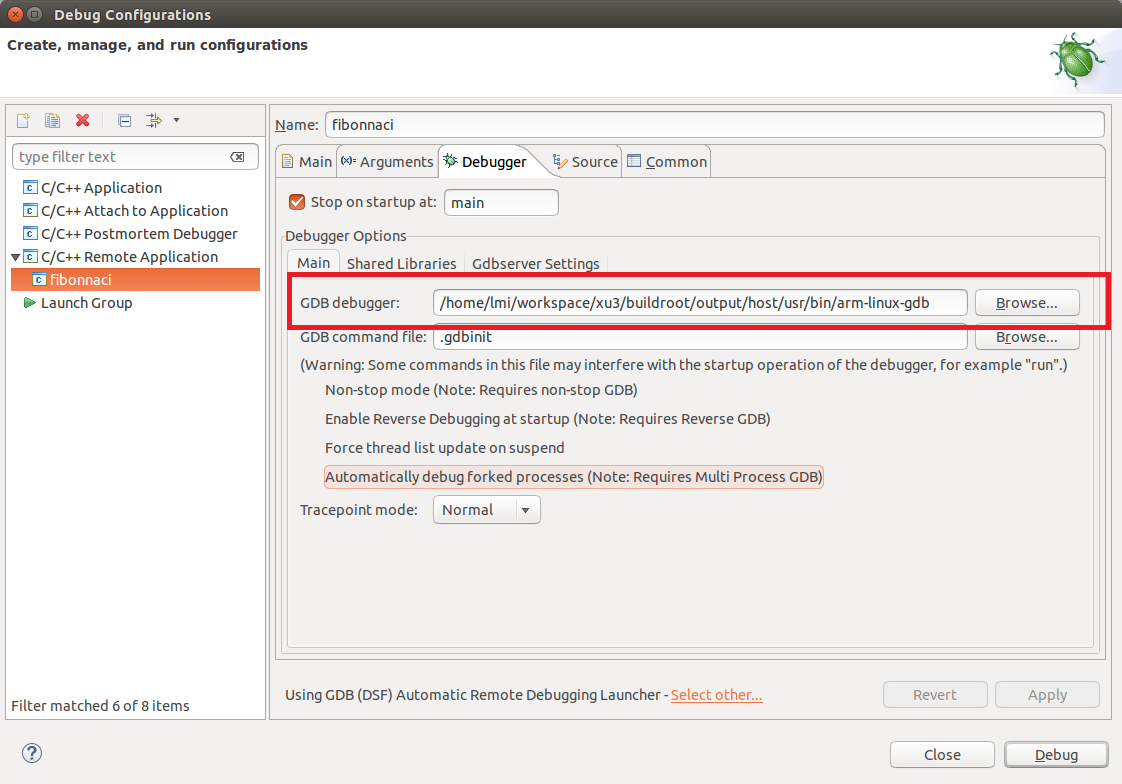
\includegraphics[width=15cm]{img/eclipseConfig3.png}
		\caption{Configuration du server gdb}
		\label{eclipseConfig3}
	\end{center}
\end{figure}
\begin{figure}[H]
	\begin{center}
		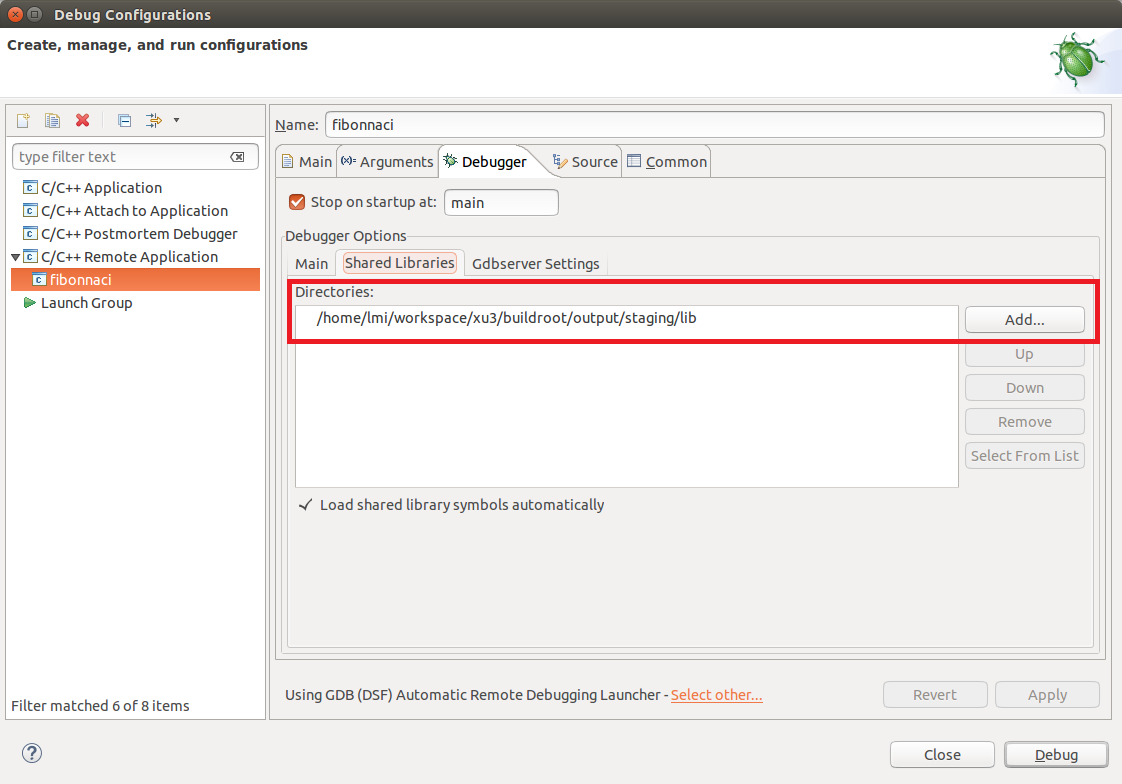
\includegraphics[width=16cm]{img/eclipseConfig4.png}
		\caption{Configuration des shared library}
		\label{eclipseConfig4}
	\end{center}
\end{figure}
Avec cette configuration, on peut ensuite debugger pas à pas les exercices d’exemples. Voici un exemple avec fibonacci:
\begin{figure}[H]
	\begin{center}
		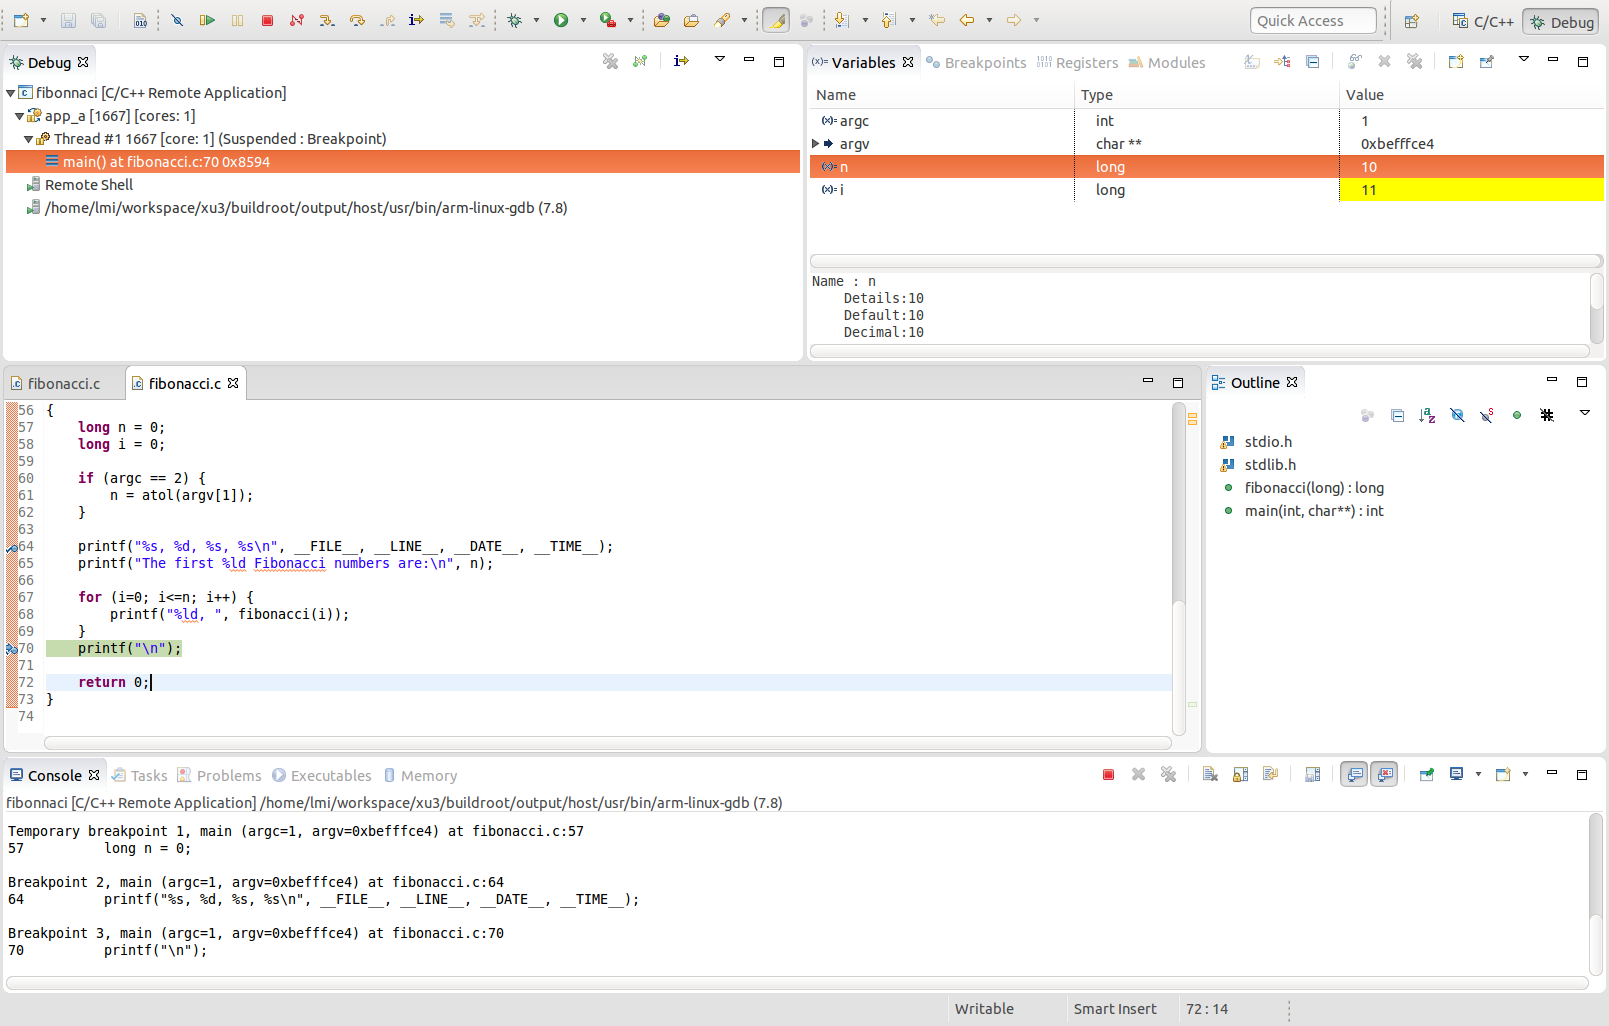
\includegraphics[width=16.5cm]{img/eclipseConfig5.png}
		\caption{Debug de l'exemple Fibonacci}
		\label{eclipseConfig5}
	\end{center}
\end{figure}
\subsection{Travail à réaliser}
\begin{enumerate}
	\item Installer l'environnement de développement sur la machine hôte, selon les instructions ci-dessus, et configurer la cible en mode de développement avec NFS sous Eclipse.\\Installer/configurer SSH pour accès à distance.
	\item Créer un script permettant de générer la carte SD.
	\item Configurer le noyau Linux afin de mounter un usrfs sous ext4 depuis la carte SD. Ce dernier sera monté dans le répertoire "/usr/local/".
	\item Tester les différentes méthodes et techniques de débogage proposées par l'environnement Linux. Pour cela générer les exemples fournis dans le répertoire "~/workspace/csel1/environement/" en suivant les indications des slides.
	\item Sur la base de l'exercice 4, mettre l'ODROID-XU3 en mode production. Un petit programme situé dans le "usrfs" sera démarré au lancement de la cible.
\end{enumerate}
À ce point du rapport, les points 1 et 2 ont déjà été réalisés.
\subsection{Configuration du noyau pour monter un usrfs}
Le usrfs ou user file system est une des partitions que nous avons créée sur la carte SD. Le usrfs peut contenir des programmes spécifiques à une application de la plateform. Il est possible de monter cette partition dans un répertoire de notre choix, ici "/usr/local". Pour monter le usrfs, il suffit de taper les commandes suivantes sur la cible:
\begin{lstlisting}
# mkdir /usr/local
# mount -t ext4 /dev/mmcblk0p2 /usr/local
\end{lstlisting}
"mmcblk0p2" indique le bloc mémoire 0 partition 2. Si l'on regarder la configuration de la carte SD faite plus haut, c'est à cette endroit que l'on a placé le usrfs.\\
Si l'on veut que ce montage se fasse automatiquement au démarrage de la cible, il faut d'ajouter au fichier \textit{/etc/fstab} la ligne suivante:
\begin{lstlisting}
/dev/mmcblk0p2 /usr/local ext4 defaults 0 0
\end{lstlisting}
Il faut ensuite activer la configuration, redémarrer et vérifier que le montage s'est fait correctement:
\begin{lstlisting}
# mount -a
# reboot
...
# mount                                                                         
...
/dev/mmcblk0p2 on /usr/local type ext4 (rw,relatime,data=ordered)      
\end{lstlisting}

\subsection{Test des différents exemples proposés}
Pour la suite du rapport, les symboles suivant sont définis:
\begin{enumerate}
	\item \$ : commande sur la machine hôte
	\item \# : commande sur la cible
	\item > : commande sur la cible arrêtée avant démarrage
\end{enumerate}

\subsubsection{Fibonacci}
\begin{lstlisting}
lmi@csel1:~/workspace/csel1/environment/samples/fibonacci$ make clean all

lmi@csel1:~$ ssh root@192.168.0.11
# cd ../usr/workspace/csel1/environment/samples/fibonacci/
# ./app_a 10
fibonacci.c, 64, Oct 31 2015, 15:27:54
The first 10 Fibonacci numbers are:
0, 1, 1, 2, 3, 5, 8, 13, 21, 34, 55,
\end{lstlisting}

\subsubsection{Tracing}
Avec la trace active
\begin{lstlisting}
lmi@csel1:~/workspace/csel1/environment/samples/tracing$ make DEBUG=1 clean all

# cd ../tracing/
# ./app_a 12
fibonacci.c, 70, Oct 31 2015, 15:35:42
The first 12 Fibonacci numbers are:
0, 1, 1, 2, 3, 5, 8, 13, 21, 34, 55, 89, 144, 
\end{lstlisting}
Avec la trace inactive
\begin{lstlisting}
lmi@csel1:~/workspace/csel1/environment/samples/tracing$ make clean all

# ./app_a 12
The first 12 Fibonacci numbers are:
0, 1, 1, 2, 3, 5, 8, 13, 21, 34, 55, 89, 144, 
\end{lstlisting}

\subsubsection{Core dumps}
\begin{lstlisting}
lmi@csel1:~/workspace/csel1/environment/samples/core_dumps$ make clean all

# cd ../core_dumps/
# ulimit -c unlimited
# ./app_a 
Segmentation fault (core dumped)
# gdb app_a core
...
Core was generated by `./app_a'.
Program terminated with signal SIGSEGV, Segmentation fault.
#0  0x000083e0 in access_data () at core_dumps.c:31
31		*p=10;
(gdb) bt
#0  0x000083e0 in access_data () at core_dumps.c:31
#1  0x00008424 in call (n=0) at core_dumps.c:37
#2  0x00008420 in call (n=1) at core_dumps.c:36
#3  0x00008420 in call (n=2) at core_dumps.c:36
#4  0x00008420 in call (n=3) at core_dumps.c:36
#5  0x00008420 in call (n=4) at core_dumps.c:36
#6  0x00008420 in call (n=5) at core_dumps.c:36
#7  0x00008420 in call (n=6) at core_dumps.c:36
#8  0x00008420 in call (n=7) at core_dumps.c:36
#9  0x00008420 in call (n=8) at core_dumps.c:36
#10 0x00008420 in call (n=9) at core_dumps.c:36
#11 0x00008420 in call (n=10) at core_dumps.c:36
#12 0x00008448 in main () at core_dumps.c:43
\end{lstlisting}


\subsubsection{Backtrace}
Cet exemple s'effectue uniquement sur la machine hôte
\begin{lstlisting}
lmi@csel1:~/workspace/csel1/environment/samples/core_dumps$ cd ../backtrace/
lmi@csel1:~/workspace/csel1/environment/samples/backtrace$ make clean all
...
lmi@csel1:~/workspace/csel1/environment/samples/backtrace$ ./app_h
backtrace() returned 17 addresses
./app_h[0x80484fc]
[0xb7727404]
./app_h[0x804854a]
./app_h[0x8048571]
./app_h[0x804856c]
./app_h[0x804856c]
./app_h[0x804856c]
./app_h[0x804856c]
./app_h[0x804856c]
./app_h[0x804856c]
./app_h[0x804856c]
./app_h[0x804856c]
./app_h[0x804856c]
./app_h[0x804856c]
./app_h[0x804859c]
/lib/i386-linux-gnu/libc.so.6(__libc_start_main+0xf3)[0xb757ca83]
./app_h[0x8048401]
Segmentation fault (core dumped)
lmi@csel1:~/workspace/csel1/environment/samples/backtrace$ addr2line -e app_h 0x804859c
/home/lmi/workspace/csel1/environment/samples/backtrace/main.c:61

\end{lstlisting}
\subsubsection{System calls}
\begin{lstlisting}
lmi@csel1:~/workspace/csel1/environment/samples/system_calls$ make clean all

# cd ../system_calls/
# ./app_a
current temperature: 46.00 degree Celcius

# strace ./app_a
execve("./app_a", ["./app_a"], [/* 21 vars */]) = 0
brk(0)                                  = 0x11000
...
+++ exited with 0 +++

# strace -e trace=mmap2 ./app_a
...
mmap2(NULL, 4096, PROT_READ|PROT_WRITE, MAP_PRIVATE|MAP_ANONYMOUS, -1, 0) = 0xb6ff9000
mmap2(NULL, 4096, PROT_READ|PROT_WRITE, MAP_PRIVATE|MAP_ANONYMOUS, -1, 0) = 0xb6ffa000
current temperature: 47.00 degree Celcius
+++ exited with 0 +++
\end{lstlisting}

\subsubsection{Memory leaks}
\begin{lstlisting}
lmi@csel1:~/workspace/csel1/environment/samples/memory_leaks$ make clean all

# cd ../memory_leaks/
# ./app_a 
# valgrind --leak-check=full ./app_a
==1714== Memcheck, a memory error detector
==1714== Copyright (C) 2002-2013, and GNU GPL'd, by Julian Seward et al.
==1714== Using Valgrind-3.10.0 and LibVEX; rerun with -h for copyright info
==1714== Command: ./app_a
==1714== 
==1714== 
==1714== HEAP SUMMARY:
==1714==     in use at exit: 31,880 bytes in 3,985 blocks
==1714==   total heap usage: 4,000 allocs, 15 frees, 32,000 bytes allocated
==1714== 
==1714== 31,880 (8 direct, 31,872 indirect) bytes in 1 blocks are definitely lost in loss record 2 of 2
==1714==    at 0x483535C: malloc (in /usr/lib/valgrind/vgpreload_memcheck-arm-linux.so)
==1714== 
==1714== LEAK SUMMARY:
==1714==    definitely lost: 8 bytes in 1 blocks
==1714==    indirectly lost: 31,872 bytes in 3,984 blocks
==1714==      possibly lost: 0 bytes in 0 blocks
==1714==    still reachable: 0 bytes in 0 blocks
==1714==         suppressed: 0 bytes in 0 blocks
==1714== 
==1714== For counts of detected and suppressed errors, rerun with: -v
==1714== ERROR SUMMARY: 1 errors from 1 contexts (suppressed: 0 from 0)
\end{lstlisting}

\subsection{Mise en production de l'ODROID-XU3}

Le fichier S60appl a été légèrement modifié pour que le path vers app\_a corresponde:
\begin{lstlisting}
#!/bin/sh
#
# Daemon application
#
case "$1" in
	start)
		/usr/workspace/csel1/environment/samples/daemon/app_a
		;;
	stop)
		killall app_a
		;;
	restart|reload)
		killall app_a
		/usr/workspace/csel1/environment/samples/daemon/app_a
		;;
	*)
		echo $"Usage: $0 {start|stop|restart}"
		exit 1
esac

echo "Daemon application launched"

exit $?
\end{lstlisting}
Il suffit ensuite de copier ce fichier dans \textit{/etc/init.d} et de faire un reboot. Au démarrage de la cible, le script \textit{/etc/init.d/rcs} va effectuer tous les fichiers S?? présent dans le répertoire \textit{/etc/init.d}, donc notre application également.
\begin{lstlisting}
# cp /usr/workspace/csel1/environment/samples/daemon/S60appl /etc/init.d
#reboot
...
Starting logging: OK                                                            
Starting mdev...                                                                
Initializing random number generator... done.                                   
Starting network...                                                             
ip: RTNETLINK answers: File exists                                              
Starting sshd: OK                                                               
Daemon application launched                                                     
[    9.933833] [c4] pwm-samsung: tin parent at 66600000  
\end{lstlisting}
\newpage
\color{red}
\subsection{Réponse aux questions}
1. Comment faut-il procéder pour générer l'U-Boot?
\begin{lstlisting}

\end{lstlisting}
2. Comment peut-on ajouter et générer un package supplémentaire dans le Buildroot?
\begin{lstlisting}

\end{lstlisting}
3. Comment doit-on procéder pour modifier la configuration du noyau Linux?
\begin{lstlisting}

\end{lstlisting}
4. Comment faut-il faire pour générer son propre RootFS?
\begin{lstlisting}

\end{lstlisting}
5. Comment faut-il procéder pour utiliser la carte eMMC en lieu et place de la carte SD?
\begin{lstlisting}

\end{lstlisting}
\color{black}

